%
%===============>>  ПРОБНИК 1 <<=============
%

%BEGIN_FOLD % ====>>_____ Вариант 1 _____<<====
\begin{training}[1]
	\title{Часть 1}
	\begin{listofex}
		%1
		\item Для объектов, указанных в таблице, определите, какими цифрами они обозначены на схеме. Заполните таблицу, в ответ запишите последовательность четырёх цифр.
			\begin{center}
			\footnotesize
			\begin{tabular}{|g|c|c|c|c|}
				\hline
				\textbf{Объекты}&Туалет&Детская&Гостиная&Кухня\\
				\hline
				\textbf{Цифры}&&&&\\
				\hline
			\end{tabular}
		\end{center}
			На плане изображена схема квартиры (сторона каждой клетки на схеме равна \( 1 \) м). Вход и выход осуществляются через единственную дверь.\\			
			При входе в квартиру расположен коридор, отмеченный цифрой \( 1 \). Напротив входа расположена туалетная комната, а справа от нее --- ванная комната.\\			
			Гостиная занимает наибольшую площадь в квартире, а справа от неё находится кухня. Прямо перед гостиной находится детская. Из детской можно попасть на балкон, отмеченный цифрой \( 6 \).\\
			Потолок в гостиной планируется покрасить в красный цвет. Для покраски одного м\( ^2 \) потолка требуется \( 0,25 \) л краски.\\
			В квартире планируется установить счётчик электроэнергии. Имеется возможность установить однотарифный или двухтарифный счётчик.
		\gapwidth
		\begin{center}
			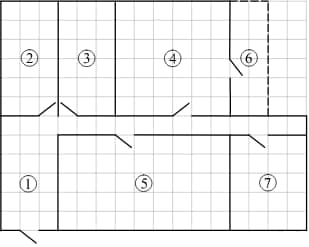
\includegraphics[align=t, width=0.5\linewidth]{\picpath/prob_2.2_1}
		\end{center}
		%2
		\item Краска продаётся в банках по \( 3 \) л. Сколько банок краски требуется купить, чтобы покрасить потолок в гостиной?
			\foranswer
		%3
		\item Найдите площадь, которую занимают детская и балкон. Ответ дайте в квадратных метрах.
		\foranswer
		%4
		\item Найдите расстояние между противоположными углами детской комнаты в метрах. Ответ запишите в виде \( \dfrac{d}{\sqrt{2}} \).
		%5
		\item 
			Хозяин квартиры планирует установить в квартире счётчик. Он рассматривает два варианта: однотарифный или двухтарифный счётчики. Цены на оборудование и стоимость его установки, данные о потребляемой мощности, и тарифах оплаты даны в таблице.
			Обдумав оба варианта, хозяин решил установить двухтарифный электросчётчик. Через сколько дней непрерывного использования электричества экономия от использования двухтарифного счётчика вместо однотарифного компенсирует разность в стоимости установки двухтарифного счётчика и однотарифного?
			\foranswer
		\gapwidth
		\begin{center}
			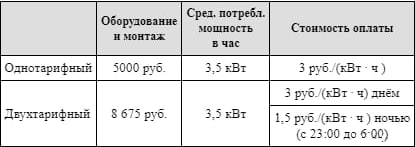
\includegraphics[align=t, width=0.8\linewidth]{\picpath/prob_2.2_2}
		\end{center}
		%6
		\item Найдите значение выражения: \( 2,5\cdot3,5-0,35 \)
		\foranswer
		%7
		\item Известно, что \( 0<a<1 \). Выберите наименьшее из чисел. В ответе укажите номер правильного ответа.
		\begin{tasks}(4)
			\task \( a^2 \)
			\task \( a^3 \)
			\task \( -a \)
			\task \( \dfrac{1}{a} \)
		\end{tasks}
		\foranswer
		%8
		\item Найдите значение выражения \( \sqrt{7\cdot3^4}\cdot\sqrt{7\cdot2^2} \).
		\foranswer
		%9
		\item Решите уравнение \(2-3(2x+2)=5-4x\)
		\foranswer
		\hphantom{Часть 1}
		%10
		\item На  тарелке  лежат  пирожки,  одинаковые  на  вид:  \(4\)  с  мясом,  \(8\)  с  капустой  и \(3\) с яблоками. Петя наугад выбирает один пирожок. Найдите вероятность того, что пирожок окажется с яблоками
		\foranswer
		%11
		\item На одном из рисунков изображен график функции \( y=x^2-2x+3 \). Укажите номер этого рисунка.
		\begin{center}
			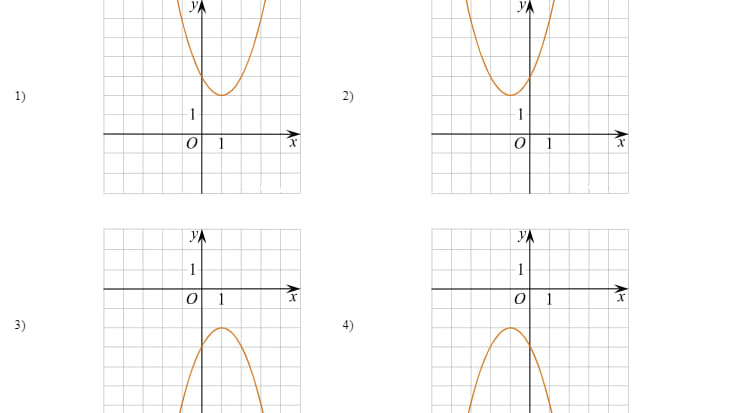
\includegraphics[align=t, width=0.8\linewidth]{\picpath/prob_2.2_4}
		\end{center}
		\foranswer
		%12
		\item Площадь четырёхугольника можно вычислить по формуле \\ \( S=\dfrac{d_1d_2\sin\alpha}{2} \),  где \( d_1 \) и \( d_2 \) --- длины диагоналей четырёхугольника, \( \alpha \) --- угол между диагоналями. Пользуясь этой формулой, найдите длину диагонали \( d_2 \), если \( d_1=6 \), \( \sin\alpha=\dfrac{1}{11} \), а \( S=3 \).
		\foranswer
			\end{listofex}
		\newpage
		\begin{listofex}[resume]
		%13
		\item На каком рисунке изображено множество решений неравенства\\ \( (2x-5)(x+3)\ge0 \)? В ответе укажите номер правильного варианта.
		\begin{center}
			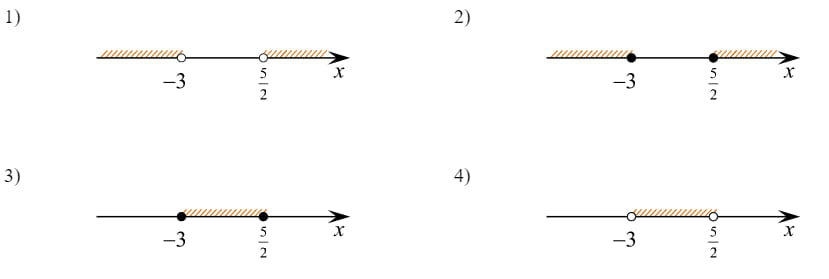
\includegraphics[align=t, width=0.9\linewidth]{\picpath/prob_2.2_6}
		\end{center}
		\foranswer
		%14
		\item Камень бросают в глубокое ущелье. При этом в первую секунду он пролетает \( 15 \) метров, а в каждую следующую секунду на \( 10 \) метров больше, чем в предыдущую, до тех пор, пока не достигнет дна ущелья. Сколько метров пролетит камень за первые четыре секунды?
		\foranswer
		%15
		\item \begin{minipage}[t]{\bodywidth}
			В равнобедренной трапеции известна высота, меньшее основание и угол при основании. Найдите большее основание.
			\foranswer
		\end{minipage}
		\gapwidth
		\begin{minipage}[t]{\picwidth}
			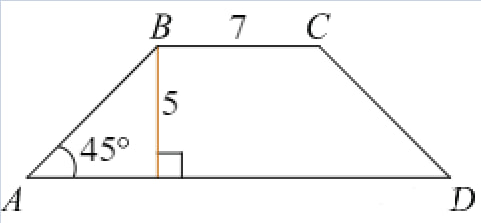
\includegraphics[align=t, width=\linewidth]{\picpath/prob_2.2_8}
		\end{minipage}
		%16
		\item \begin{minipage}[t]{\bodywidth}
			Найдите \( \angle DEF \), если градусные меры дуг \( DE \) и \( EF \) равны \( 150\degree \) и \( 68\degree \) соответственно.
			\foranswer
		\end{minipage}
		\gapwidth
		\begin{minipage}[t]{\picwidth}
			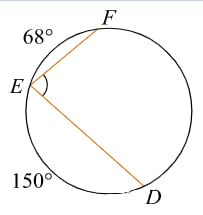
\includegraphics[align=t, width=\linewidth]{\picpath/prob_2.2_10}
		\end{minipage}
		%17
		\item \begin{minipage}[t]{\bodywidth}
		В треугольнике \( ABC \) \( DE \) --- средняя линия. Площадь треугольника \( CDE \) равна \( 9 \). Найдите площадь треугольника \( ABC \).
			\foranswer
		\end{minipage}
		\gapwidth
		\begin{minipage}[t]{\picwidth}
			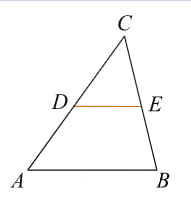
\includegraphics[align=t, width=\linewidth]{\picpath/prob_2.2_11}
		\end{minipage}
		%18
		\item \begin{minipage}[t]{\bodywidth}
			На клетчатой бумаге с размером клетки \( 1\times1 \) изображён треугольник. Найдите его площадь.
			\foranswer
		\end{minipage}
		\gapwidth
		\begin{minipage}[t]{\picwidth}
			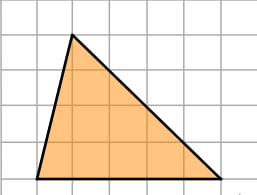
\includegraphics[align=t, width=\linewidth]{\picpath/prob_2.2_13}
		\end{minipage}
		%19
		\item Какие из следующих утверждений верны?
		\begin{tasks}(1)
			\task Через точку, не лежащую на данной прямой, можно провести прямую, параллельную этой
			 прямой.
			 \task Треугольник со сторонами \( 1 \), \( 2 \), \( 4 \) существует.
			 \task В любом параллелограмме есть два равных угла.
		\end{tasks}
		\foranswer
		\title{Часть 2}
		%20
		\item Сократите дробь \( \dfrac{75^n}{5^{2n-1}\cdot3^{n-2}} \)
		%21
		\item Теплоход проходит по течению реки до пункта назначения \( 280 \) км и после стоянки возвращается в пункт отправления. Найдите скорость теплохода в неподвижной воде, если скорость течения равна \( 4 \) км/ч, стоянка длится \( 15 \) часов, а в пункт отправления теплоход возвращается через \( 39 \) часов после отплытия из него.
		%22
		\item Постройте график функции \( y=\dfrac{(x^2+2,25)(x-1)}{1-x} \) и определите, при каких значениях \( k \) прямая \( y=kx \) имеет с графиком ровно одну общую точку.
		%23
		\item Основания трапеции равны \( 16 \) и \( 34 \). Найдите отрезок, соединяющий середины диагоналей трапеции.
		%24
		\item В параллелограмме \( ABCD \) проведены высоты \( BH \) и \( BE \) к сторонам \( AD \) и \( CD \) соответственно, при этом \( BH=BE \). Докажите, что \( ABCD \) --- ромб.
		%25
		\item Основание \( AC \) равнобедренного треугольника \( ABC \) равно \( 10 \). Окружность радиуса \( 7,5 \) \( \, \) с центром вне этого треугольника касается продолжения боковых сторон треугольника и касается основания \( AC \) в его середине. Найдите радиус окружности, вписанной в треугольник \( ABC \).
	\end{listofex}
\end{training}
%END_FOLD

%BEGIN_FOLD % ====>>_____ Вариант 2 _____<<====
\begin{training}[2]
	\title{Часть 1}
	\begin{listofex}
		%1
		\item
		На рисунке точками показано количество минут исходящих вызовов и трафик мобильного интернета в гигабайтах, израсходованных абонентом в процессе пользования смартфоном, за каждый месяц \(2019\) года. Для удобства точки, соответствующие минутам и гигабайтам, соединены сплошными и пунктирными линиями соответственно.
			\foranswer
		\gapwidth
		\begin{center}
			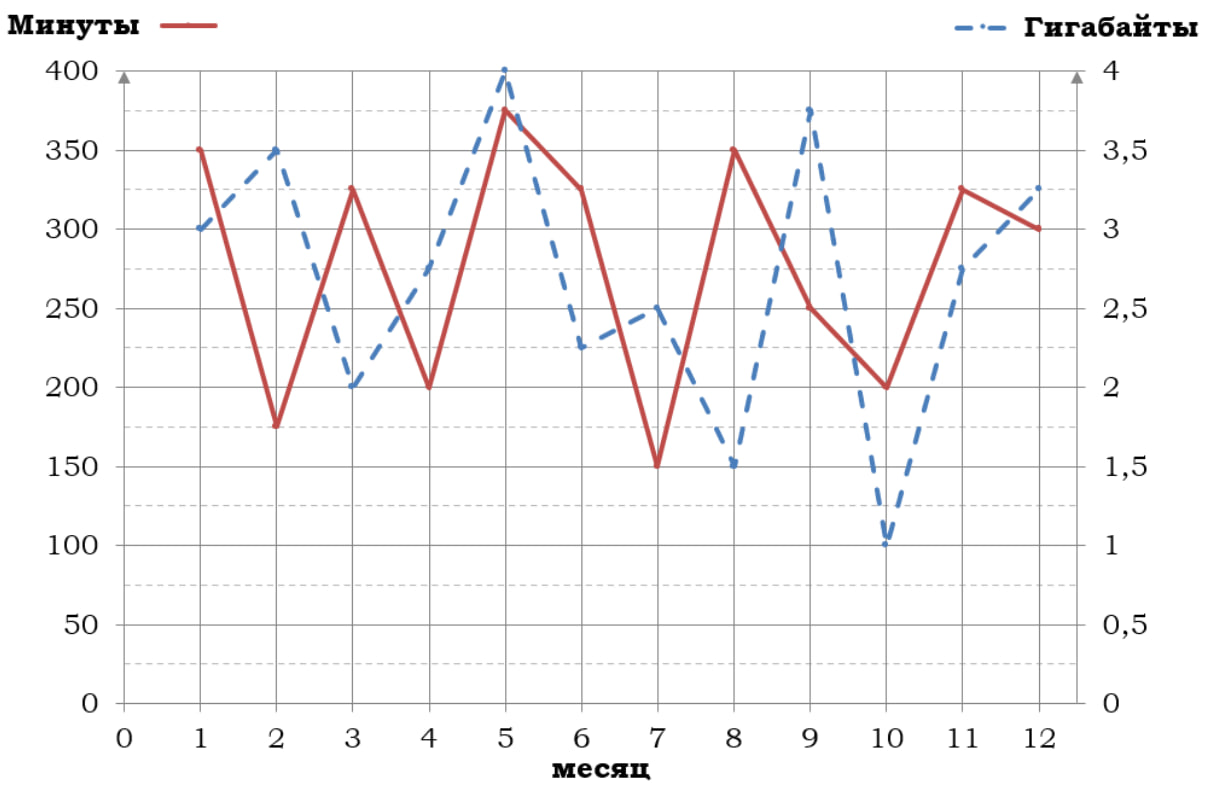
\includegraphics[align=t, width=\linewidth]{\picpath/prob_23_91}
		\end{center}\\
		В течение года абонент пользовался тарифом «Стандартный», абонентская плата по которому составляла \(380\) рублей в месяц. При условии нахождения абонента на территории РФ в абонентскую плату тарифа «Стандартный» входит:
		\begin{itemize}
			\item пакет минут, включающий \(300\) минут исходящих вызовов на номера, 	зарегистрированные на территории РФ;
			\item пакет интернета, включающий \(3\) гигабайта мобильного интернета;
			\item пакет SMS, включающий \(120\) SMS в месяц;
			\item безлимитные бесплатные входящие вызовы.
		\end{itemize}
		Стоимость минут, интернета и SMS сверх пакета тарифа указана в таблице.
		\begin{center}
			\begin{tabular}{ |c|c| }
				\hline
				Исходящие вызовы & \(3\) руб./мин. \\ 
				\hline
				Мобильный интернет (пакет) & \(80\) руб. за \(0,5\) ГБ \\
				\hline
				SMS & \(2\) руб./шт. \\
				\hline
			\end{tabular}
		\end{center}
		Абонент не пользовался услугами связи в роуминге. За весь год абонент отправил \(110\) SMS.\\
		 Пользуясь рисунком, поставьте в соответствие каждому из указанных периодов времени характеристику израсходованных минут и гигабайтов
		\begin{center}
			\begin{tabular}{ |p{1.7in}|p{2.8in}| }
				\hline
				\textbf{Периоды} & \textbf{Характеристики} \\ 
				\hline
				\textbf{А)} март --- апрель & \textbf{1)} расход минут увеличился, а расход
				гигабайтов уменьшился\\
				\hline
				\textbf{Б)} апрель --- май & \textbf{2)} расход гигабайтов увеличился, а
				расход минут уменьшился\\
				\hline
				\textbf{В)} сентябрь --- октябрь & \textbf{3)} расход минут увеличился и расход гигабайтов увеличился
\\
				\hline
				\textbf{Г)} июль --- август & \textbf{4)} расход минут уменьшился и расход гигабайтов уменьшился\\
				\hline
			\end{tabular}
		\end{center}
		В таблице под каждой буквой укажите соответствующий номер. В ответ запишите последовательность цифр без пробелов, запятых и других дополнительных символов.
		\foranswer
		%2
		\item Сколько рублей потратил абонент на услуги связи в декабре? 
		\foranswer
		%3
		\item Сколько месяцев в 2019 году абонент превысил лимит по пакету мобильного интернета? 
		\foranswer
		%4
		\item На сколько процентов увеличилось количество минут исходящих вызовов в ноябре по сравнению с октябрём 2019 года?
		\foranswer
		%5
		\item Помимо мобильного интернета, абонент использует домашний интернет от провайдера «Омега». Этот интернет-провайдер предлагает три тарифных плана. Условия приведены в таблице.
	\begin{center}
		\begin{tabular}{ |p{1in}|p{1.6in}|p{1.6in}| }
			\hline
			Тарифный план & Абонентская плата & Плата за трафик \\ 
			\hline
			"0" & Нет & 1,4 руб. за 1 Мб \\
			\hline
			"300" & 315 руб. за 300 Мб трафика в месяц & 1,2 руб. за 1 Мб сверх 300 Мб \\
			\hline
			"800" & 950 руб. за 800 Мб трафика в месяц & 0,5 руб. за 1 Мб сверх 800 Мб \\
			\hline
		\end{tabular}
	\end{center}
	Абонент предполагает, что трафик составит 800 Мб в месяц, и выбирает наиболее дешёвый тарифный план. Сколько рублей должен будет заплатить абонент за месяц, если трафик действительно будет равен 800 Мб?
		\foranswer
		%6
		\item Найдите значение выражения: \( \dfrac{11}{4,4\cdot2,5} \).
		\foranswer
		%7
		\item Какое из данных чисел принадлежит промежутку \( [7;8] \)? В ответ укажите номер правильного варианта.
		\begin{tasks}(4)
			\task \( \sqrt{7} \)
			\task \( \sqrt{8} \)
			\task \( \sqrt{48} \)
			\task \( \sqrt{56} \)
		\end{tasks}
		\foranswer
		%8
		\item Найдите значение выражения \( (4+\sqrt{5})^2+(4-\sqrt{5})^2 \)
		\foranswer
		\newpage
		%9
		\item Решите уравнение: \(x^2+x-12=0\).\\
		Если уравнение имеет более одного корня, в ответ запишите больший из корней
		\foranswer
		%10
		\item Телевизор у Васи сломался и показывает только один случайный канал. Вася включает телевизор. В это время по восемнадцати каналам из тридцати показывают кинокомедии. Найдите вероятность того, что Вася попадет на канал, где комедия не идет.
		\foranswer
		%11
		\item График какой из приведённых ниже функций изображён на рисунке?
		\begin{center}
			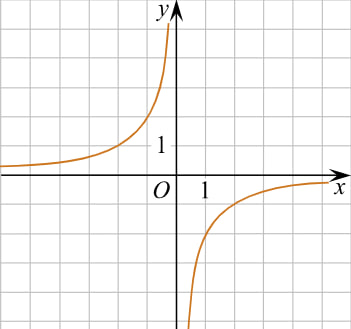
\includegraphics[align=t, width=0.5\linewidth]{\picpath/prob_2.2_5}
		\end{center}
		\begin{tasks}(4)
			\task \( y=-\dfrac{2}{x} \)
			\task \( y=\dfrac{2}{x} \)
			\task \( y=-\dfrac{1}{2x} \)
			\task \( y=\dfrac{1}{2x} \)
		\end{tasks}
		\foranswer
		%12
		\item Площадь четырёхугольника можно вычислить по формуле \\ \( S=\dfrac{d_1d_2\sin\alpha}{2} \),  где \( d_1 \) и \( d_2 \) --- длины диагоналей четырёхугольника, \( \alpha \) --- угол между диагоналями. Пользуясь этой формулой, найдите длину диагонали \( d_2 \), если \( d_1=6 \), \( \sin\alpha=\dfrac{1}{11} \), а \( S=3 \).
		\foranswer
		%13
		\item Решите неравенство \( x^2-4x<0 \). В ответ укажите номер правильного ответа.
		\begin{tasks}(1)
			\task \( [0;4] \)
			\task \( (-\infty;0)\cup(4;+\infty) \)
			\task \( (0;4) \)
			\task \( (-\infty;0]\cup[4;+\infty) \)
		\end{tasks}
		\foranswer
		%14
		\item У Светы есть попрыгунчик (каучуковый шарик). Она со всей силы бросила его об асфальт. После первого отскока попрыгунчик подлетел на высоту \( 560 \) см, а после каждого следующего отскока от асфальта подлетал на высоту в два раза меньше предыдущей. После какого по счёту отскока высота, на которую подлетит попрыгунчик, станет меньше \( 20 \) см?
		\foranswer
		%15
		\item
		\begin{minipage}[t]{\bodywidth}
			Тангенс острого угла прямоугольной трапеции равен \( \dfrac{5}{6} \).  Найдите её большее основание, если меньшее основание равно высоте и равно \( 15 \).
			\foranswer
		\end{minipage}
		\gapwidth
		\begin{minipage}[t]{\picwidth}
			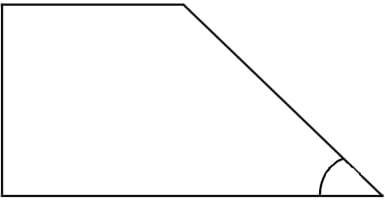
\includegraphics[align=t, width=\linewidth]{\picpath/prob_2.2_7}
		\end{minipage}
		%16
		\item 
		\begin{minipage}[t]{\bodywidth}
			Прямая касается окружности в точке \( K \). Точка \( O \) --- центр окружности. Хорда \( KM \) образует с касательной угол, равный \( 75\degree \). Найдите величину угла \( OMK \). Ответ дайте в градусах.
			\foranswer
		\end{minipage}
		\gapwidth
		\begin{minipage}[t]{\picwidth}
			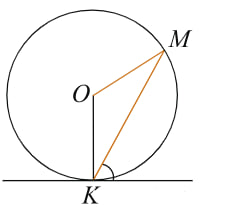
\includegraphics[align=t, width=\linewidth]{\picpath/prob_2.2_9}
		\end{minipage}
		%17
		\item Основания трапеции равны \( 18 \) и \( 12 \), одна из боковых сторон равна \( 6 \), а синус угла между ней и одним из оснований равен \( \dfrac{1}{3} \).  Найдите площадь трапеции.
		\foranswer
		%18
		\item \begin{minipage}[t]{\bodywidth}
			На рисунке изображен параллелограмм \( ABCD \). Используя рисунок, найдите \( \sin\angle HBA \).
			\foranswer
		\end{minipage}
		\gapwidth
		\begin{minipage}[t]{\picwidth}
			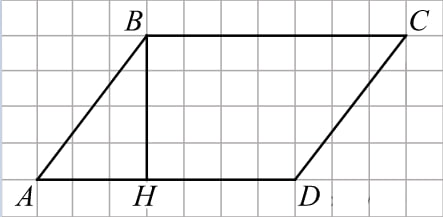
\includegraphics[align=t, width=\linewidth]{\picpath/prob_2.2_12}
		\end{minipage}
		%19
		\item Какие из следующих утверждений верны?
		\begin{tasks}(1)
			\task Любые два прямоугольных треугольника подобны.
			\task Если катет и гипотенуза прямоугольного треугольника равны соответственно \( 6 \) и \( 10 \), то второй катет этого треугольника равен \( 8 \).
			\task Стороны треугольника пропорциональны косинусам противолежащих углов.
			\task Квадрат любой стороны треугольника равен сумме квадратов двух других сторон без удвоенного произведения этих сторон на косинус угла между ними.
		\end{tasks}
		\foranswer
		\title{Часть 2}
		%20
		\item Решите уравнение \( (x^2-9)^2+(x^2-2x-15)^2=0 \)
		%21
		\item При смешивании первого раствора кислоты, концентрация которого \( 20\% \), и второго раствора этой же кислоты, концентрация которого \( 50\% \), получили раствор, содержащий \( 30\% \) кислоты. В каком отношении были взяты первый и второй растворы?
		%22
		\item Постройте график функции
		\[y= \left\{
		\begin{array}{l}
			x-3, \quad x<3,\\
			-1,5x+4,5,\quad 3\le x\le4,\\
			1,5x-7,5, \quad x>4,
		\end{array}
		\right.\]
		и определите, при каких значениях \( m \) прямая \( y=m \) имеет с графиком ровно две общие точки.
		%23
		\item Основания трапеции равны \( 16 \) и \( 34 \). Найдите отрезок, соединяющий середины диагоналей трапеции.
		%24
		\item На медиане \( KF \) треугольника \( MKP \) отмечена точка \( E \). Докажите, что если \( EM=EP \), то \( KM=KP \).
		%25
		\item Основание \( AC \) равнобедренного треугольника \( ABC \) равно \( 10 \). Окружность радиуса \( 7,5 \) \( \, \) с центром вне этого треугольника касается продолжения боковых сторон треугольника и касается основания \( AC \) в его середине. Найдите радиус окружности, вписанной в треугольник \( ABC \).
	\end{listofex}
\end{training}
%END_FOLD